
\documentclass[]{spie}

% Package imports go here.
\renewcommand{\baselinestretch}{1.0} % Change to 1.65 for double spacing

\usepackage{amsmath,amsfonts,amssymb}
\usepackage{graphicx}
\usepackage[colorlinks=true, allcolors=blue]{hyperref}
\usepackage{listings}
\usepackage{xcolor}
\usepackage{longtable}

% Local commands go here.
\newcommand{\aj}{AJ}
\newcommand{\apj}{ApJ}
\newcommand{\apjs}{ApJS}
\newcommand{\procspie}{Proc.\ SPIE}
\newcommand{\pasj}{PASJ}
% lsstdoc documentation: https://lsst-texmf.lsst.io/lsstdoc.html
\input{meta}

% Package imports go here.

% Local commands go here.

% See ASPmanual2010.pdf 2.1.4  and ManuscriptInstructions.pdf for more details
%\markboth{auth}{short title}


\newcommand{\docRef}{DMTN-343}
\newcommand{\docUpstreamLocation}{\url{https://github.com/lsst-dm/dmtn-343}}


\begin{document}
\input{authors}
\title{Observing the Observatory. The Observability Journey of the Vera C. Rubin Observatory}

% This can write metadata into the PDF.
% Update keywords and author information as necessary.
\hypersetup{
    pdftitle={Observing the Observatory. The Observability Journey of the Vera C. Rubin Observatory},
    pdfauthor={silvac},
    pdfkeywords={}
}

\maketitle


\begin{abstract}
The Vera C. Rubin Observatory is not only an observatory, it is also a distributed production engine for science. During operations, it will move thousands of images, metadata, and alerts through the telescope, camera, network, storage, and processing services every night. Rubin will produce up to 20 TB of raw data per night (10TB on the wire with compression), with an alert stream that reaches millions of events and a target latency of nearly 1 minute \cite{2019ApJ...873..111I}.

In this environment, simple monitoring is not enough. We need to ask why something changed, where latency started, which component is under pressure, and whether the behavior is connected with the observing conditions or the state of the facility. This paper describes the observability journey of the Vera C. Rubin Observatory DevOps team, a multi-year effort to build, refine, and scale a modern observability stack for one of the most ambitious astronomical facilities ever constructed.

The platform is based on open-source components, and the result is, not only a software stack, it is an operations model. Dashboards and alerts are treated as code; labels are part of the interface between teams; and the observability system is continuously improved as commissioning and operations reveal new questions. The paper highlights dashboard creation strategies, discusses the hard parts: configuration complexity, label discipline, storage and retention trade-offs, human adoption, and the need to keep improving the system rather than calling it finished \cite{lsst-it-k8s-cookbook}.
\end{abstract}



\section{Introduction}

Rubin Observatory is being built to observe the sky repeatedly and rapidly. This creates a
different type of operations problem. The observing system must work as one chain: telescope and
camera, summit and base infrastructure, high-speed networks, storage systems, computing clusters,
databases, control services, and data processing services. If one part of the chain is slow or
becomes unstable, the effect can be seen elsewhere. A storage problem can look like an application
problem. A network issue can look like a data-acquisition issue. A problem in a tiny computing
process can affect a dashboard used by a scientist or an operator during the night.

Hence we made the observability platform part of the observatory itself. We are observing the
system that observes the sky. To conduct reliable scientific operations, we need to view the
observatory with the same seriousness with which we view the sky.

Rubin Observatory will push up to 10\,TB of data through the pipeline every night, triggering
millions of alerts \cite{rubin-dm,rubin-keynumbers,rubin-alerts}. Therefore, decisions have to
happen fast; there is no time to wait when the next image is arriving in 34 seconds. A minute lost
chasing down a graph is a minute the telescope cannot get back.

The observability system described in this paper is not a whiteboard architecture; it reflects
years of operational experience, shaped by real incidents, evolving requirements, and the kind of
hard-won knowledge that only comes from running infrastructure under pressure. The design decisions
made capture not just what was built, but also how the team thinks about keeping environments
consistent and ensuring changes are traceable \cite{lsst-it-k8s-cookbook}.

\section{From Monitoring to Observability}

A traditional monitoring system usually starts with simple questions. Is the service up? Is the
disk full? Is the CPU high? These questions are necessary, but they are not enough for a facility
like Rubin. Observability enables understanding of a system's internal behavior from the signals it
emits. In Kubernetes, observability is typically built from metrics, logs, and traces, along with
the tools that make them usable for operators \cite{kubernetes-observability}.

The practical difference is important. Monitoring can tell us that an alert pipeline is slow.
Observability should help us decide whether the reason is the Kafka broker, the network, the
storage layer, an overloaded Kubernetes node, an ingress problem, a database, or something related
to the observing sequence. Monitoring can indicate that a pod has restarted; observability should
help us understand what changed around that time, who was affected, and what to check next.

Our approach is also a journey. The current platform is not the first iteration we tried, and it
will not be the last. The important part is that the platform became more reproducible and easier
to inspect over time.

At the beginning, we did what most teams do: we installed Icinga and set it up for basic up/down
checks. It was a reasonable first step, but it did not take long to realize that a platform of this
complexity could not be understood solely through availability probes. We could see things were
failing, but we had no insight into why.

Among the team, we had backgrounds with Nagios, Zabbix, Zenoss, and even HP OpenView, and more,
but none of those felt like the right direction. We decided that open-source tools were the right
choice, not because they are free of cost, but because they can be operated, modified, and
connected to the rest of the observatory without vendor lock-in.

We knew we needed outside help to build a modern observability stack, so we hired a contractor.
One of their consultants was an active maintainer of Prometheus, which gave us confidence that we
were talking to the right people.

We wrote down our requirements and handed them over. What we learned over the following months is
that our environment is genuinely unusual. Our components come from many different vendors and do
not follow any standard pattern. That made everything slower and harder to implement than either
side expected. It took close to two years before the contractor delivered something we could call
substantial. Even then, we were never happy with the logging side. They had gone with OpenSearch,
and while we understood the reasoning, it never felt like a good fit for us. It was not well
integrated with Grafana, and the resource consumption was hard to justify. The dashboards were also
a source of friction. We eventually came to understand that part of the problem was our own
requirements; we had asked for dashboards built around a preconceived idea of what should be shown,
when in reality dashboards need to be driven by what is actually happening in the infrastructure,
not the other way around.

When the contract ended, we took the chance to redo the logging from scratch. We picked Loki,
mostly because it is part of the Grafana Labs ecosystem and fits naturally with everything else we
were already running. That choice felt like the moment we stopped working around someone else's
observability architecture and started building something that actually made sense for us.

\section{Requirements and Design Principles}

The requirements for the platform came from two directions. On the technology side, we needed
scalable ingestion, long retention, Kubernetes-native service discovery, log aggregation, alerting,
and dashboards. On the operations side, the need was harder to pin down but just as important: a
common language between teams. A graph is only useful when the right people understand what it
means and what to do next. On top of that, our infrastructure spans many types of hardware from
different vendors, each with its own quirks, and our users have very different expectations of what
the platform should show them. That diversity made the dashboard design particularly difficult;
there was no single answer that worked for everyone.

The DevOps operations rely on a set of core design principles, and any observability stack we built
had to reflect them from the ground up \cite{lsst-it-k8s-cookbook,prometheus-operator,grafana-loki-alloy,grafana-loki}.

\begin{center}
\begin{minipage}{\linewidth}
\renewcommand{\arraystretch}{1.3}
\small
\textbf{Table 1. Core Design Principles and Their Operational Rationale}\\[4pt]
\begin{tabular}{p{0.22\linewidth} p{0.36\linewidth} p{0.32\linewidth}}
\hline
\textbf{Principle} & \textbf{Implementation pattern in the platform} & \textbf{Why it matters for operations} \\
\hline
\textbf{Configuration as code} &
  Keep dashboards, alert rules, Helm values, and overlays in Git. &
  Changes are reviewed, promoted, and recovered like the rest of the infrastructure. \\[4pt]
\textbf{Open-source first} &
  Use Prometheus, Grafana, Loki, Mimir, Alloy, Fleet, exporters, and Kubernetes ecosystem tools. &
  The team can inspect the system, tune it, and avoid a single vendor dependency. \\[4pt]
\textbf{Kubernetes-native discovery} &
  Use ServiceMonitor, PodMonitor, Probe, and label selectors. &
  Teams can onboard services using conventions rather than one-off manual edits. \\[4pt]
\textbf{Multi-site and multi-cluster awareness} &
  Carry labels such as \texttt{site} and \texttt{cluster} into metrics and logs. &
  Operators can compare behavior across environments and avoid guessing where a signal came from. \\[4pt]
\textbf{Logs and metrics together} &
  Collect Kubernetes logs, node logs, events, and metrics into systems that can be queried from Grafana. &
  Incidents usually need both time-series trends and exact log messages. \\[4pt]
\textbf{Room for constant improvement} &
  Treat dashboards and alerts as living assets, not as a finished project. &
  Commissioning and operations create new questions, so the platform must keep changing. \\
\hline
\end{tabular}
\end{minipage}
\end{center}

\section{Platform Architecture}

The observability platform is not a single monitoring tool. It is a distributed system where each
environment produces its own signals: metrics from nodes, workloads, and control-plane components;
logs from pods and hosts; cluster events; and telemetry from storage, networking, Kafka, databases,
and facility services. Those signals are collected close to where they are produced, tagged with
site and cluster context, and made available through shared backends and dashboards.

\subsection{Metrics}

Metrics start close to where things happen. Kubernetes components, nodes, workloads, network
devices, storage systems, and applications all produce time-series data. The platform collects this
through a combination of exporters and monitors, some built into the stack, some added for specific
systems like SNMP devices or facility services.

Prometheus handles the collection and short-term storage. It scrapes targets, evaluates alert
rules, and makes metrics available for immediate incident response
\cite{lsst-it-k8s-cookbook,prometheus-operator,prometheus-alerting}. The configuration is adapted
for Rubin, with the right labels, selectors, and alerting choices, but the underlying tooling comes
from the Prometheus ecosystem, which is widely used and well understood.

For anything beyond the short incident-response window, Mimir provides long-term storage. It is a
horizontally scalable backend that speaks the same query language as Prometheus, so the experience
for operators and dashboard authors does not change \cite{grafana-mimir}. Under the hood, it uses
object storage and runs as a distributed service with separate components for ingestion, querying,
compaction, and caching.

This gives the team two distinct capabilities. Recent metrics support fast triage---you can see
what is happening right now and what changed in the last hour. Older metrics support a different
kind of question: how does tonight compare to last month? Is this cluster behaving differently from
the others? Is this a new problem or a slow drift that has been building for weeks? That longer
view is especially important during commissioning, when the baseline is still being established and
slow changes are easy to miss.


\subsection{Logs}

Alloy runs close to the nodes and collects host logs, pod logs, and cluster events. Before sending
anything to Loki, it enriches each log line with metadata: namespace, pod, container, application,
severity \cite{lsst-it-k8s-cookbook,grafana-loki-alloy}. 

\begin{lstlisting}[
    basicstyle=\ttfamily\small,
    breaklines=true,
    frame=single,
    backgroundcolor=\color{gray!10},
    rulecolor=\color{gray!50},
    caption={Alloy relabeling configuration for Kubernetes events}
]
loki.process "cluster_events" {
    forward_to = [loki.write.send.receiver]
    stage.static_labels {
      values = {
        cluster = "${ get .ClusterLabels "management.cattle.io/cluster-display-name" }",
      }
    }
    stage.regex {
      expression = ".*name=(?P<name>[^ ]+).*kind=(?P<kind>[^ ]+).*objectAPIversion=(?P<apiVersion>[^ ]+).*type=(?P<type>[^ ]+).*"
    }
    stage.labels {
      values = {
        name       = "name",
        kind       = "kind",
        apiVersion = "apiVersion",
        type       = "type",
      }
    }
  }
\end{lstlisting}

But Kubernetes is not the only source.
Network devices, firewalls, power systems, and other facility equipment connected to the observatory
network also send logs, and those flow into the same pipeline. Loki. 

Loki stores logs differently from a traditional log system. Instead of indexing the full content
of each line, it indexes labels and stores the log chunks compressed in object storage
\cite{grafana-loki}. This keeps costs manageable at scale, but it requires some discipline: too
few labels and queries become slow and broad; too many dynamic labels and the index grows in ways
that hurt performance. Getting that balance right is part of the design work, not something that
happens automatically.

The deployment is not a minimal installation. It runs in distributed mode with gateways, separate
ingesters and queriers, object storage, retention policies, rate limits, and caches
\cite{lsst-it-k8s-cookbook}. This is not complexity for its own sake; during a real observing
night, logs are only useful if they can be queried quickly and if the labels are good enough to
narrow the search fast.

The deeper point is that logs and metrics need to be designed together, not as separate systems
that happen to run on the same cluster. A metric can tell you that latency spiked at a specific
time. A log query can show what the service was reporting at that exact moment. A Kubernetes event
can show that a pod was restarting. A network log can show a device dropping packets. None of those
signals alone tells the full story. The operator needs the timeline, and building that timeline is
only possible if the signals share a common labeling scheme and a common sense of time.

\subsection{Dashboards}

The dashboard collection is one of the most visible parts of the platform. There are dashboards for
Kubernetes, storage, networking, Kafka, logging, power devices, databases, and service checks
\cite{lsst-it-k8s-cookbook}. Each one encodes a question that someone needed to answer during an
incident or a commissioning shift.

The breadth matters. Observability cannot stop at application pods. The systems that enable
scientific operations all need to be visible in the same place. Dashboards need to let operators
move across those layers without losing their train of thought.

The collection also includes more local, informal dashboards, built because someone needed to
answer a specific question and the general dashboards were not enough. That is a healthy sign. A
living platform has both the polished general views that everyone uses and the rougher tools that
someone built. Over time, the useful ones get promoted into the standard set.

\begin{center}
    \begin{minipage}{0.7\linewidth}
        \centering
        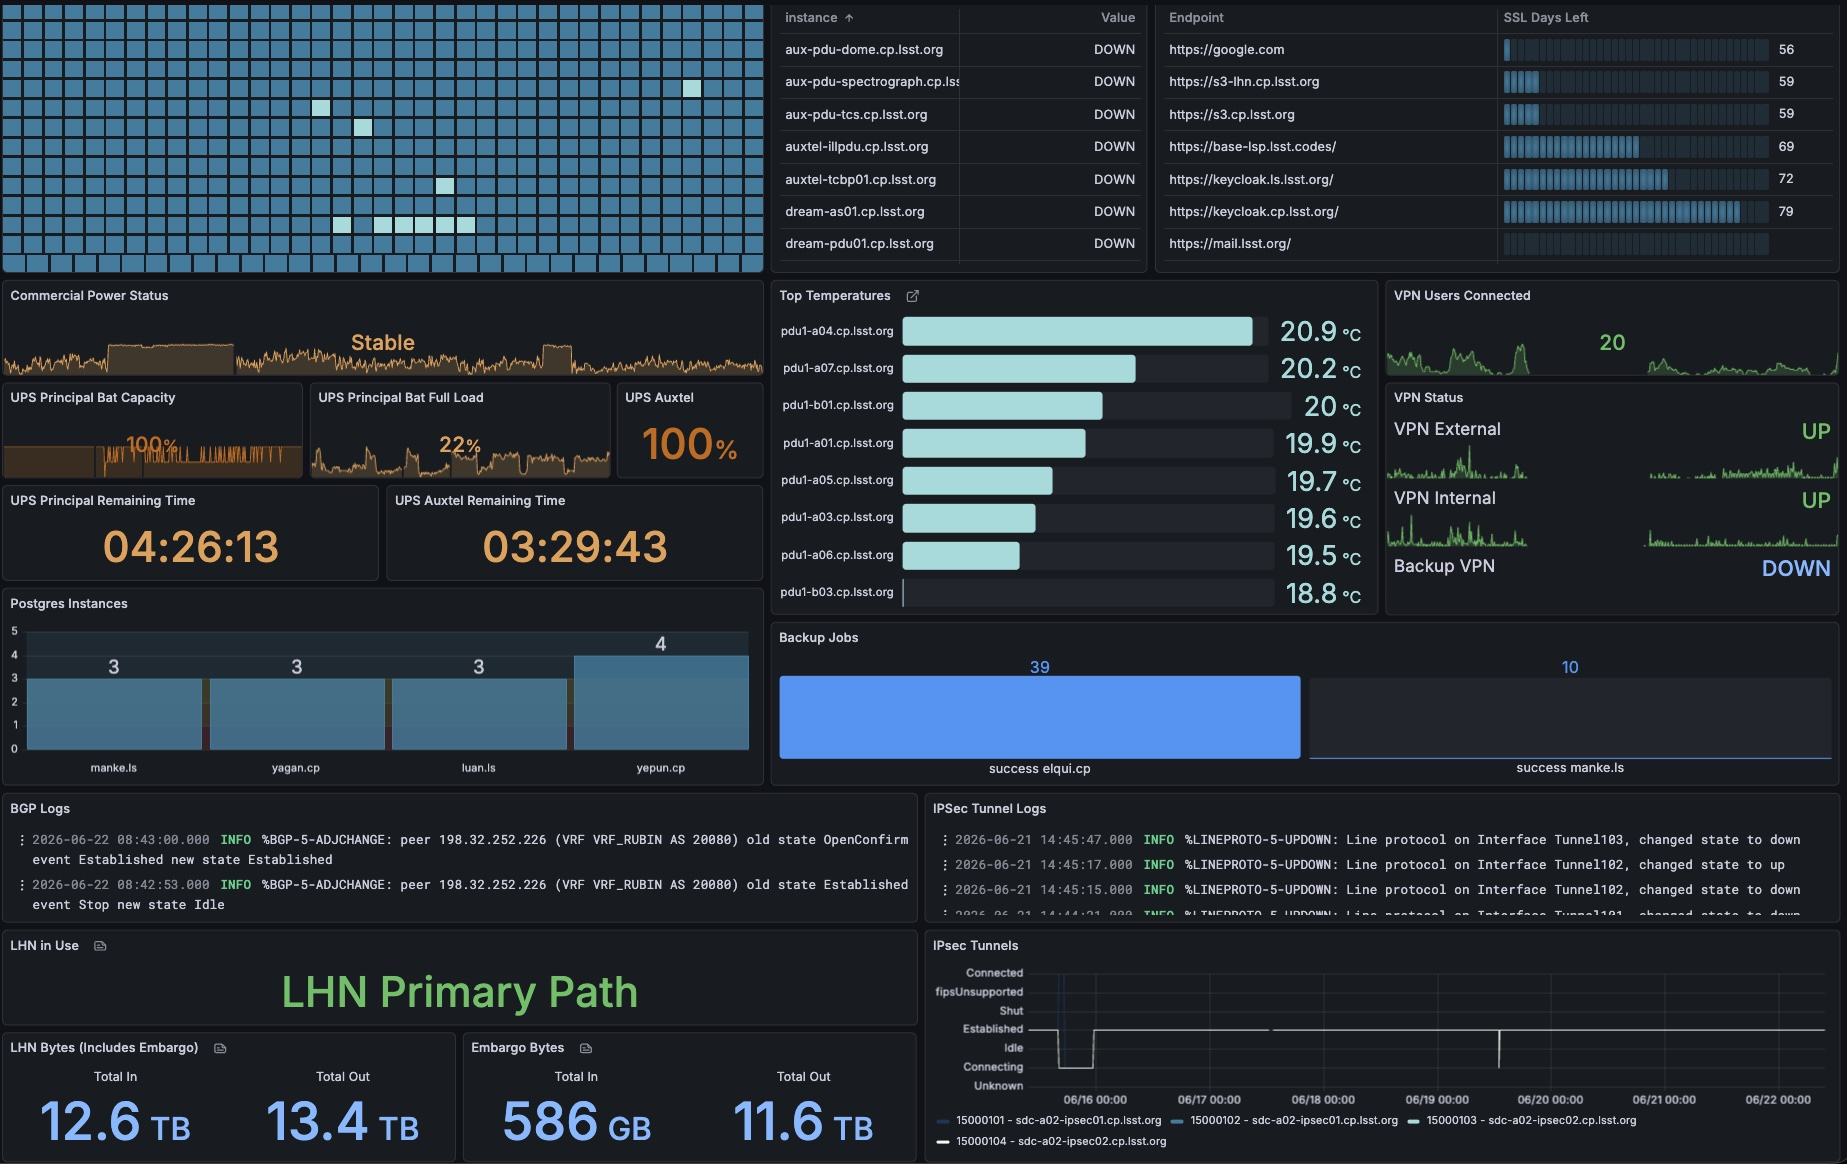
\includegraphics[width=\linewidth]{spie_dashboard.jpg}
        \\[4pt]
        \textbf{Figure 1.} Summary dashboard of several useful metrics for Engineers and Operators.
    \end{minipage}
\end{center}

One deliberate choice in the dashboard design is color. Every palette used across the dashboards
was selected to be readable under all common forms of color blindness \cite{wcag-color}. This is
not a cosmetic detail; it is an operational requirement. It does not matter how much information a
dashboard contains if the person looking at it cannot immediately tell that something is wrong, or
cannot distinguish between two states at a glance. Any engineer, operator, or scientist at the
observatory should be able to look at a panel and read it correctly, regardless of how they
perceive color.

The difference becomes clear when you simulate how the same dashboard looks under different visual
conditions. Under deuteranopia and protanopia, the two most common forms of red-green color
blindness, the conventional red/green palette collapses \cite{wcag-color}. Red and green become
nearly identical shades of brownish yellow. An operator glancing at the panel during a busy night
has no quick visual cue; they have to stop and read the label to know whether something is up or
down. That extra second matters when you are watching twenty panels at once.

\begin{center}
    \begin{minipage}{0.7\linewidth}
        \centering
        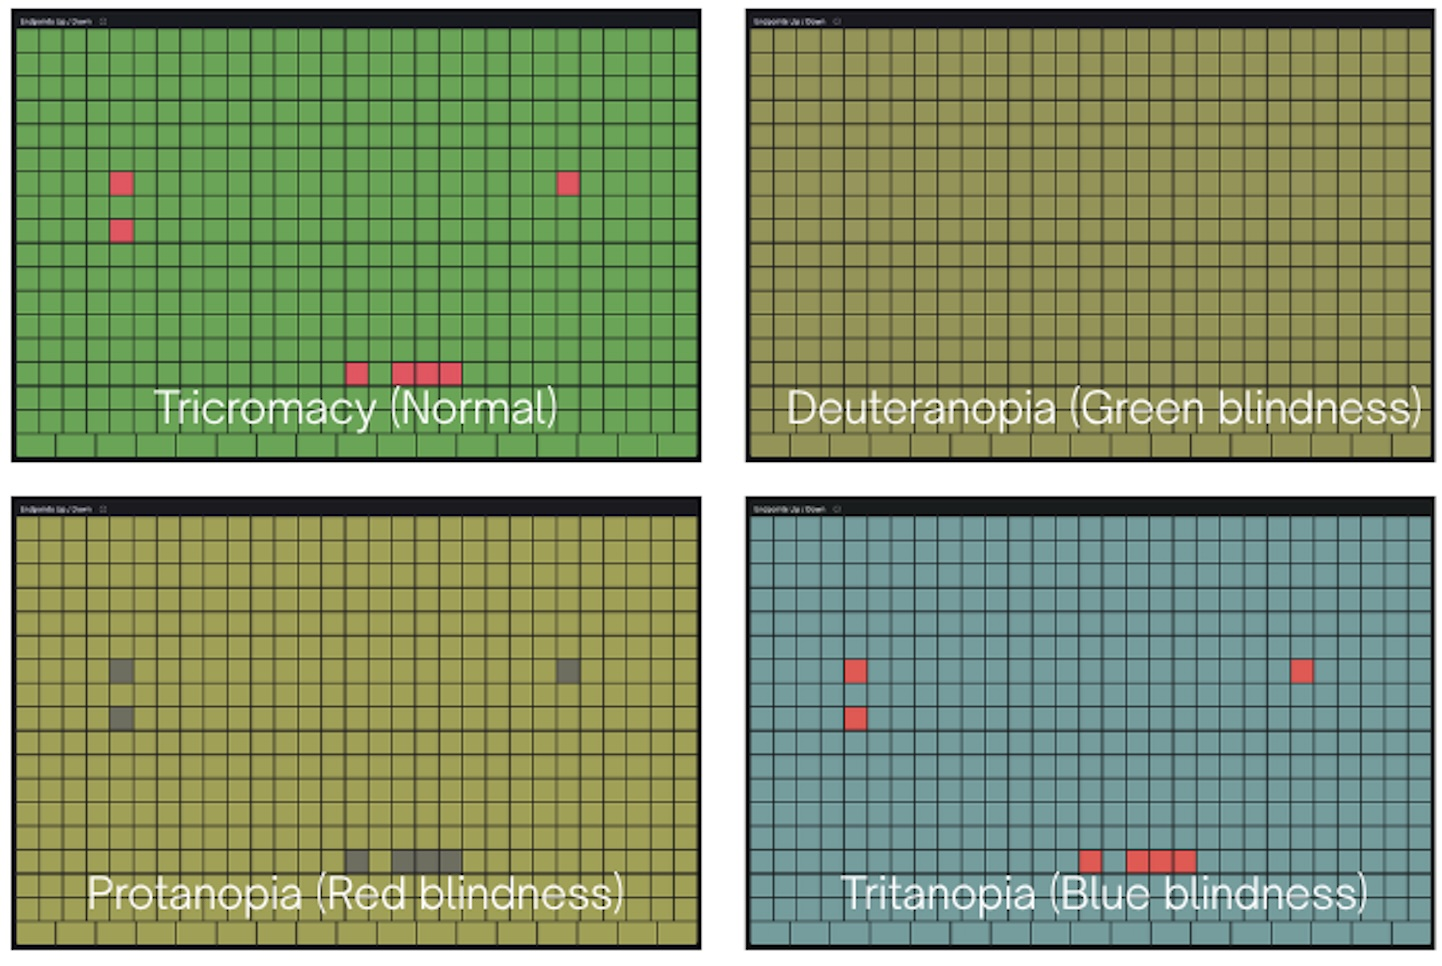
\includegraphics[width=\linewidth]{spie_red.jpg}
        \\[4pt]
        \textbf{Figure 2.} Up and Down monitor using default red and green colors, under different forms of color blindness.
    \end{minipage}
\end{center}

With our palette, the same simulation tells a different story. The colors remain visually distinct
under all tested conditions. The contrast is preserved not only in typical vision but also in
deuteranopia, protanopia, and tritanopia. Someone who has never been able to rely on red and green
to mean anything receives the same immediate signal as everyone else.

\begin{center}
    \begin{minipage}{0.7\linewidth}
        \centering
        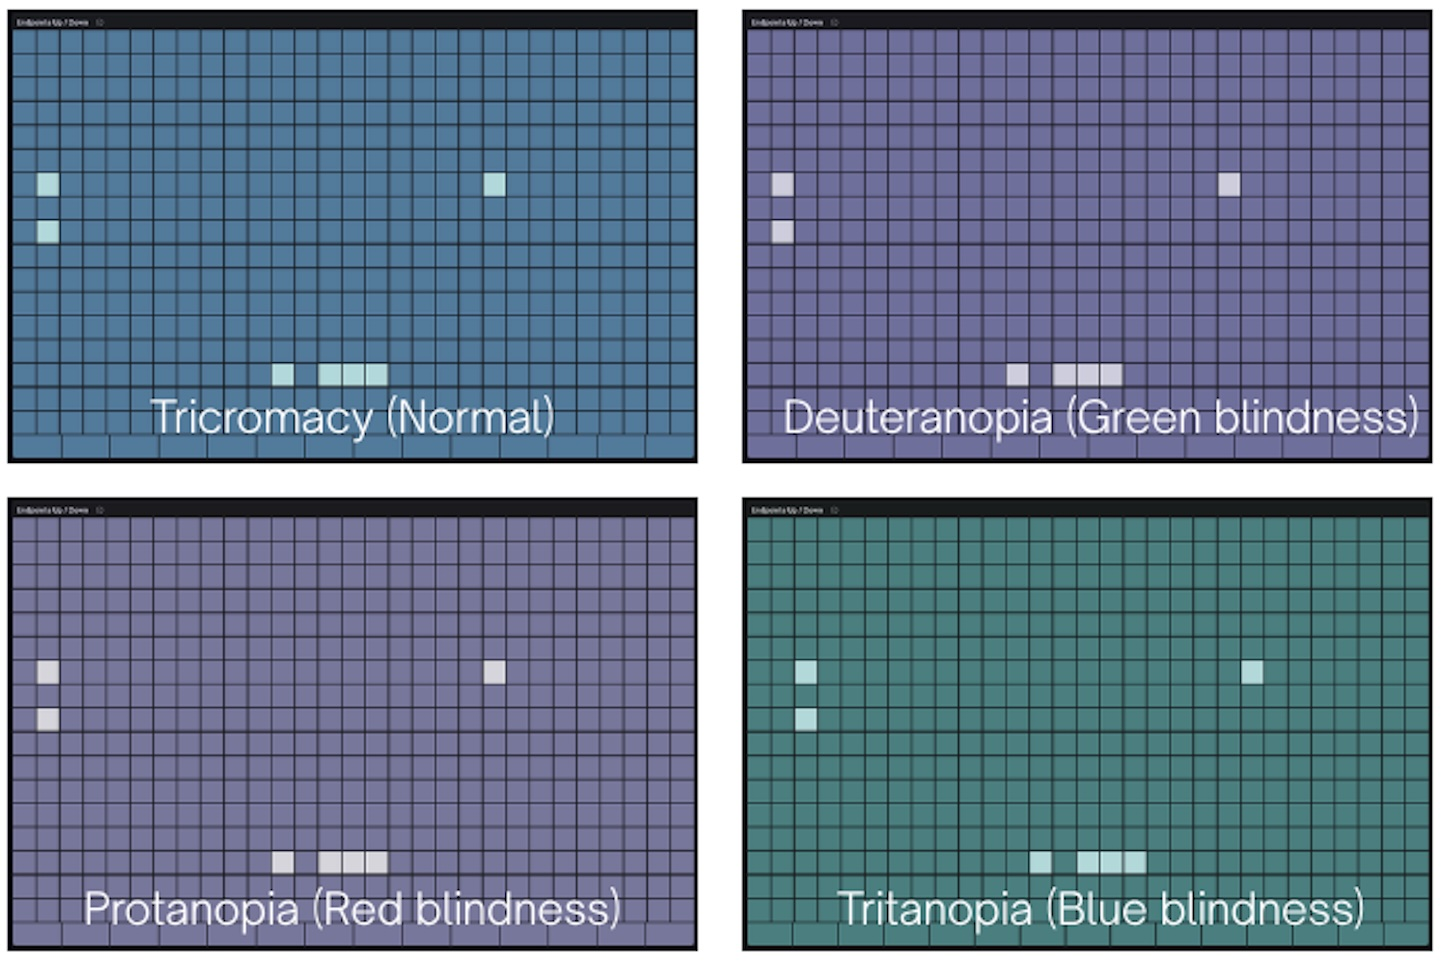
\includegraphics[width=\linewidth]{spie_nored.jpg}
        \\[4pt]
        \textbf{Figure 3.} Up and Down monitor using colors that can be noticeable under different forms of color blindness.
    \end{minipage}
\end{center}

That is the actual goal: not a palette that looks good in a screenshot, but one that works for
every person standing in front of the screens when it matters.

While this development only works with Rubin dashboards, we are exploring how to contribute this
work upstream so it can benefit the broader Grafana community.

\subsection{Alerting}

Alerts are a part of observability that interrupts people. That makes them different from
dashboards---a bad dashboard is inconvenient, but a bad alert wakes someone up at 3\,am for the
wrong reason, or worse, stays silent when something actually needs attention.

The platform stores alert rules as code, following the same review and promotion process as
everything else \cite{lsst-it-k8s-cookbook,prometheus-alerting,prometheus-alertmanager}. But the
technical side is the easier part. The harder part is writing alerts that are actually useful.

A good alert is not just a PromQL expression that fires when a number crosses a threshold
\cite{prometheus-alerting,prometheus-alertmanager}. It carries enough context to start a diagnosis:
what the condition is, how urgent it is, who should receive it, and where to look first. Without
that, an alert becomes noise, something that fires, gets acknowledged, and gets ignored. With it,
an alert is the first step of a structured response.

There is also a timing problem specific to night operations. During an observing shift, not
everything that is wrong needs immediate human attention. A saturated disk, a failed exporter, a
flapping network link, and a degraded storage component are serious, but they are not all the same
kind of serious. The alerting system needs to reflect that, routing the right signal to the right
person at the right time \cite{prometheus-alertmanager}, without flooding the on-call operator with
everything at once. Getting that routing right is ongoing work, and it improves the same way
everything else does: through real incidents, honest postmortems, and small adjustments that
accumulate over time.

\subsection{Discovery}

One of the quieter but more important parts of the platform is how it finds hosts to monitor.
There is no hand-maintained list. Instead, the platform queries the Puppet instances that manage
the observatory's infrastructure. Every time a new host is provisioned through the
infrastructure-as-code process, it becomes visible to the observability platform automatically, no
code changes, no manual additions, no tickets to update a configuration file.

This matters more than it might seem. In an environment that is still growing and changing, a
static host list becomes wrong almost immediately. A node brought up for commissioning, a host
added for a new instrument, all of them appear in the platform on their own, because the source of
truth is the infrastructure itself, not a separate list that someone has to remember to keep
current.

Services follow a different path, using Kubernetes-native discovery through label conventions. But
for the physical and virtual hosts that make up the observatory network, the answer is automatic:
provision the host, and the platform finds it.

\begin{center}
  \begin{minipage}{0.5\linewidth}
      \centering
      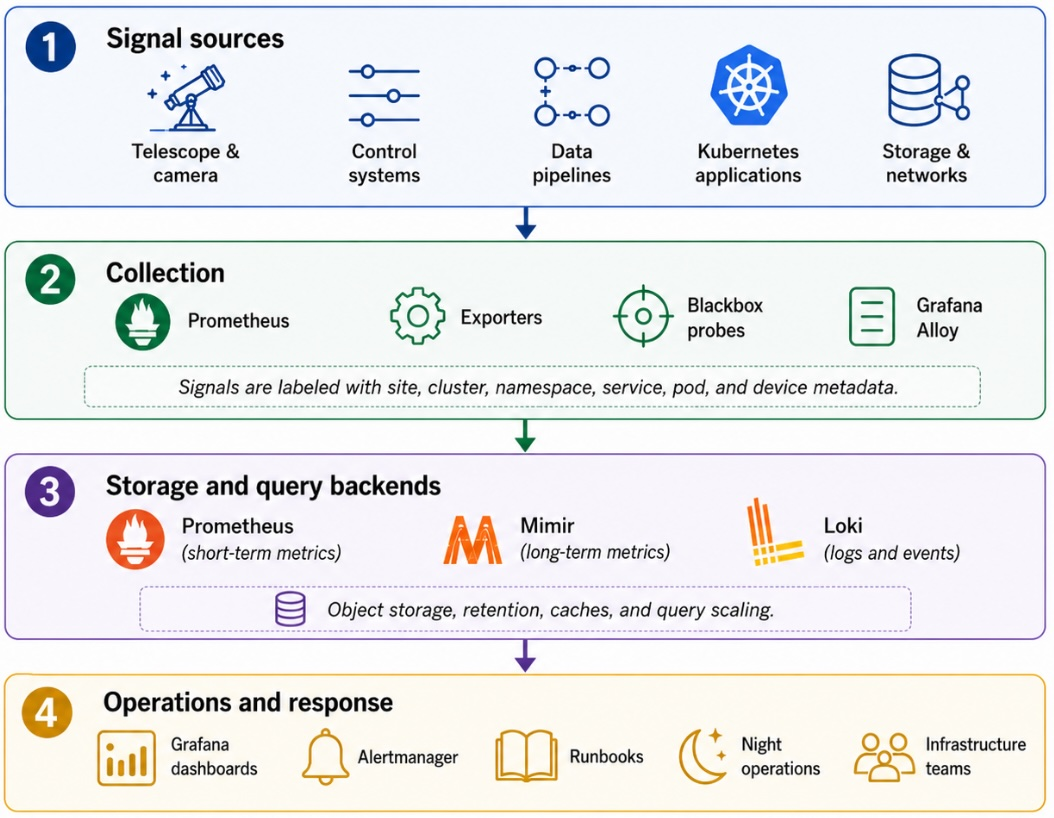
\includegraphics[width=\linewidth]{spie_arch.jpg}
      \\[4pt]
      \textbf{Figure 4.} Observability Architecture
  \end{minipage}
\end{center}% \textbf{TODO: ADD ARCHITECTURE DIAGRAM HERE}

\section{GitOps}

The platform is managed as code. Every change, a dashboard, an alert rule, the scraping
configuration, a retention policy, goes through a review process before it reaches production.
Nothing is edited directly on the cluster \cite{lsst-it-k8s-cookbook}.

Changes move through staged environments: development, testing, and production. This matters for
an observatory because you need to know not just what changed, but why. The history of every
decision is preserved and reviewable.

\subsection{Dashboards as Code}

Grafana does not natively support managing dashboards through GitOps; dashboards are normally
created and saved through the UI. To solve this, the team built a templating layer that takes
dashboard definitions from the repository and automatically deploys them to the cluster, where
Grafana picks them up \cite{lsst-it-k8s-cookbook}. This means a dashboard can be reviewed before
it goes out, reverted if it breaks something, and understood later by someone who was not there
when it was created. Dashboards are not personal views saved in someone's account; they are
operational artifacts shared by the whole team.

\subsection{Alert Rules as Code}

Prometheus has some built-in support for loading rules from files, but wiring that into a GitOps
workflow with proper staging, review, and promotion is not something that comes out of the box
\cite{lsst-it-k8s-cookbook,prometheus-alerting,prometheus-alertmanager}. The team built the same
kind of templating layer for alert rules, so they follow the same path as everything else. Each
rule carries enough context, a summary, a description, and a receiver, to be useful to whoever
gets paged at night. Rules that are vague or noisy get fixed through the same review process, so
quality improves over time.

\begin{lstlisting}[
    basicstyle=\ttfamily\small,
    breaklines=true,
    frame=single,
    backgroundcolor=\color{gray!10},
    rulecolor=\color{gray!50},
    caption={Alert rule for low PVC free space}
]
groups:
  - name: k8s.rules
    rules:
      - alert: PVCLowFreeSpace
        annotations:
          summary: PVC {{ $labels.persistentvolumeclaim }} is low on free space
          description: >
            PVC {{ $labels.persistentvolumeclaim }} in namespace {{ $labels.namespace }}
            has less than 20% free space.
        expr: |
          (kubelet_volume_stats_available_bytes{job="kubelet",metrics_path="/metrics",namespace=~".*"}
          / kubelet_volume_stats_capacity_bytes{job="kubelet",metrics_path="/metrics",namespace=~".*"}) < 0.20
          and kubelet_volume_stats_used_bytes{job="kubelet",metrics_path="/metrics",namespace=~".*"} > 0
        for: 2m
        labels:
          prod: "true"
          severity: warning
          node_name: '{{ $labels.prom_cluster }}'
          device: null
          service_name: null
\end{lstlisting}


\section{What Was Hard}

\subsection{The Complexity Is Real}

The stack has many moving parts: deployment bundles, configuration overlays, custom resources,
object storage, ingress rules, secrets, and more. This is not a small installation, and there is
no point pretending otherwise. The complexity is the cost of having a platform that covers many
systems and can still be reviewed, versioned, and rolled back.

One lesson worth stating clearly: open source does not mean low effort. It means the effort moves
to the team. Someone has to understand upgrades, chart compatibility, storage sizing, label
conventions, retention policies, and user support. That is a good trade when the team needs control
and flexibility, but it should not be described as the easy path.

\subsection{Cardinality, Retention, and Cost}

Metrics and logs grow faster than expected. Labels are essential, but labels with too many unique
values make systems slow and expensive. Logs are valuable, but high ingestion rates with long
retention eat storage quickly. Managing this is ongoing work: setting ingestion limits, tuning
retention, sizing caches, watching query performance. A slow observability system is not useful
during an incident. The platform has to stay fast enough to be trusted when it matters most.

\subsection{Human Adoption}

Dashboards are only useful when people actually use them. That requires more than good tooling; it
requires naming things clearly, showing people where to look during real problems, and revisiting
dashboards that have stopped answering relevant questions. A platform that nobody looks at during
an incident is just a collection of graphs. The social side of adoption is as important as the
technical side.

\section{What Comes Next}

The platform covers a lot of ground already, but there are clear directions where it needs to grow.

\subsection{Connecting Infrastructure to Observing Conditions}

Right now the platform is good at telling you what the infrastructure is doing. What it does not
do well yet is connect that to what the observatory is doing: which part of the observing sequence
is running, what the weather is, what state the camera and telescope are in, whether a calibration
is happening or a filter just changed. Some of that context should come in as labels. Some of it
may work better as events on a shared timeline. Either way, an operator trying to understand why
something degraded at a specific moment needs both views together, not separately.

\subsection{Tracing}

Metrics and logs cover most situations well, but there are cases---particularly in pipelines that
cross multiple services, queues, and storage systems---where it is hard to find exactly where a
request started failing. Distributed tracing can help with that \cite{opentelemetry-traces}. It is
not something to add everywhere, because it comes with instrumentation overhead and more data to
store, but in the right places it could significantly reduce the time spent finding the first
failing boundary.

\subsection{AI-Assisted Analysis}

One recent step that is already showing promise is enabling API access to Loki for developers
across the observatory. What started as a practical decision has opened up uses that go well beyond
what the dashboards were designed for. Teams are already building tools that use AI to analyze log
patterns, surface anomalies, and find correlations that would be extremely difficult to catch by
eye. The early results have been impressive. This is still the beginning, and it is hard to predict
exactly where it goes, but the direction is clear: when the data is accessible and the labels are
good, people find ways to ask questions the platform was never explicitly built to answer.

\section{Lessons Learned}

\textbf{Observability is a practice, not an installation.} The dashboards, rules, and labels that
make sense today will not all make sense in six months. The system changes, the questions change,
and the platform has to follow. Treating it as something you set up once and leave alone is how it
stops being useful.

\textbf{GitOps gives the platform memory} \cite{lsst-it-k8s-cookbook}. When a dashboard changes,
there is a reason, a review, and a record. When an alert is added or removed, the decision is
visible to anyone who looks. That history turns out to be more valuable than it seems at the time,
especially after an incident, when understanding what changed and why is exactly the question you
need to answer.

\textbf{Labels are design decisions, not metadata}
\cite{prometheus-operator,grafana-loki}. Good labels make it possible to correlate signals across
systems. Bad labels make queries slow, expensive, or just confusing. Label discipline is an
engineering interface between teams, and it deserves the same kind of care as an API.

\textbf{Seeking help from a contractor is always a good practice} when there is uncertainty about
how to move forward; however, the contractor needs very specific instructions on what to do. That
is not simple when there is little knowledge of the tools' capacity. It feels like another
contractor is needed to define the requirements to be delivered to the observability contractor.
The most reasonable approach is to give some liberty to the contractor to recommend what is best
based on their experience while maintaining very tight control over the project's progress. There
will be many situations in which requirements will be changed, added, or removed, and the
contractor needs to be aware of this. One decision that made a real difference was asking the
contractor to work alongside us rather than just deliver something. The co-work sessions gave the
team a chance to absorb how the platform was being built, why certain decisions were made, and
where the tricky parts were. By the time the contract ended, we were not starting from scratch; we
understood what we had inherited and were ready to take it further. That knowledge transfer was
probably worth as much as the platform itself.

\textbf{Dashboard work is human work.} The best dashboard is not the one with the most panels. It
is the one that helps the right person answer a question when they are tired, under pressure, and
do not have time to think. That is a harder design problem than it looks.

\textbf{Open source is a good fit when the team is ready to own it.} The transparency and
flexibility are real advantages. So is the cost: someone has to understand the upgrades, the
sizing, the edge cases, and the failure modes. For an observatory of this magnitude, that ownership is not a burden; it is part of what makes the platform
sustainable.

\section{Conclusion}

The Vera C.\ Rubin Observatory will produce science from one of the largest and fastest data
systems ever built for astronomy \cite{rubin-dm,rubin-keynumbers,rubin-alerts}. Operating that
system means being able to observe it---not just the applications, but the storage, the networks,
the facility services, and everything in between.

The platform described here is practical and continues to evolve. It is built from open-source
tools, Kubernetes conventions, and GitOps workflows, and it covers metrics, logs, dashboards, alert
rules, long-term storage, and operational views across a wide range of systems
\cite{lsst-it-k8s-cookbook,prometheus-operator,grafana-loki-alloy}. It is not finished, and it was
never meant to be.

The most important thing is not which tools were chosen. It is that the team built a way to keep
asking better questions. What changed? Where did the latency start? Which system is actually
affected? Who needs to act, and what do they need to know? What did we learn so the next night
goes more smoothly? Those questions do not stop when commissioning ends. They follow the
observatory into full operations, and the platform has to follow as well.

\acknowledgments

This material is based upon work supported in part by the National Science Foundation through Cooperative Agreements AST-1258333 and AST-2241526 and Cooperative Support Agreements AST-1202910 and AST-2211468 managed by the Association of Universities for Research in Astronomy (AURA), and the Department of Energy under Contract No.\ DE-AC02-76SF00515 with the SLAC National Accelerator Laboratory managed by Stanford University.
Additional Rubin Observatory funding comes from private donations, grants to universities, and in-kind support from LSST-DA Institutional Members.

The author notes that Anthropic Claude was used in the preparation of this paper for text formatting, proofreading, and language refinement. The underlying engineering work, technical analysis, and all conclusions presented in this paper remain entirely the authors' own.

% Include all the relevant bib files.
% https://lsst-texmf.lsst.io/lsstdoc.html#bibliographies
\bibliographystyle{spiebib}
\bibliography{local,lsst,lsst-dm,refs_ads,refs,books}

\end{document}
